%%%%%%%%%%%%%%%%%%%%%%%%%%%%%%%%%%%%%%%%%%%
%%% DOCUMENT PREAMBLE %%%
\documentclass[12pt]{report}
\usepackage[czech]{babel}
%\usepackage{natbib}
\usepackage{url}
\usepackage[utf8x]{inputenc}
\usepackage{amsmath}
\usepackage{graphicx}
\graphicspath{{images/}}
\usepackage{parskip}
\usepackage{fancyhdr}
\usepackage{vmargin}
\setmarginsrb{3 cm}{2.5 cm}{3 cm}{2.5 cm}{1 cm}{1.5 cm}{1 cm}{1.5 cm}
\usepackage{subcaption}
\title{Závislost přítomnosti poslanců na počasí}								
% Title
\author{Šimon Schierreich}						
% Author
\date{LS 2018/2019}
% Date

\makeatletter
\let\thetitle\@title
\let\theauthor\@author
\let\thedate\@date
\makeatother

\pagestyle{fancy}
\fancyhf{}
\rhead{\theauthor}
\lhead{\thetitle}
\cfoot{\thepage}
%%%%%%%%%%%%%%%%%%%%%%%%%%%%%%%%%%%%%%%%%%%%
\begin{document}

%%%%%%%%%%%%%%%%%%%%%%%%%%%%%%%%%%%%%%%%%%%%%%%%%%%%%%%%%%%%%%%%%%%%%%%%%%%%%%%%%%%%%%%%%

\begin{titlepage}
	\centering
    \vspace*{0.5 cm}
   % \includegraphics[scale = 0.075]{bsulogo.png}\\[1.0 cm]	% University Logo
\begin{center}    \textsc{\Large   České vysoké učení technické v Praze\\Fakulta informačních technologií}\\[2.0 cm]	\end{center}% University Name
	\textsc{\Large Report k semestrální práci z \textbf{MI-ADM}}\\[0.5 cm]				% Course Code
	\rule{\linewidth}{0.2 mm} \\[0.4 cm]
	{ \huge \bfseries \thetitle}\\
	\rule{\linewidth}{0.2 mm} \\[1.5 cm]
	
	\begin{minipage}{0.4\textwidth}
		\begin{flushleft} \large
			\emph{Autor:} Šimon Schierreich\\
			\emph{Semestr:} LS 2018/2019
			\end{flushleft}
			\end{minipage}~
			\begin{minipage}{0.4\textwidth}
            
			\begin{flushright} \large
			%\emph{Autor:}
		    %Šimon Schierreich 
		\end{flushright}
           
	\end{minipage}\\[7.2cm]
	
	
\includegraphics[scale = 0.35]{logo_FIT_cb.pdf}
    
    
    
    
	
\end{titlepage}

%%%%%%%%%%%%%%%%%%%%%%%%%%%%%%%%%%%%%%%%%%%%%%%%%%%%%%%%%%%%%%%%%%%%%%%%%%%%%%%%%%%%%%%%%

\tableofcontents
\pagebreak

%%%%%%%%%%%%%%%%%%%%%%%%%%%%%%%%%%%%%%%%%%%%%%%%%%%%%%%%%%%%%%%%%%%%%%%%%%%%%%%%%%%%%%%%%
\renewcommand{\thesection}{\arabic{section}}

\section{Zadání}

Zadání semestrální práce pochází od laboratoře OpenDataLab\footnote{\url{https://opendatalab.cz/}} a firmy Profinit\footnote{\url{https://www.profinit.eu}}. Cílem projektu bylo potvrdit nebo vyvrátit vztah mezi přítomností poslanců v poslanecké sněmovně a tím, jaké je počasí.

\section{Příprava dat}

V první fázi projektu bylo třeba připravit data k analýze. Navzdory tomu, že zadání pocházelo od laboratoře otevřených dat, data potřebná k další práci bohužel tak otevřená nebyla.

\subsection{Přítomnost poslanců}

Poslanecká sněmovna bohužel data ve strojově čitelném formátu neposkytuje. Na stránkách instituce jsou ovšem dostupné informace o hlasování.

Někteří analytici se již stahováním dat o hlasováních poslanců z webové prezentace sněmovny zabývali, jejich projekty jsou bohužel neaktuální. Bylo tedy třeba vytvořit vlastní web-scraper, který z webové prezentace potřebná data vytáhne. Scraper je dostupný pod open-source licencí na serveru GitHub\footnote{\url{https://github.com/opendatalabcz/weather-mp-dependency}}.

\subsection{Počasí}

V Praze existují čtyři profesionální měřící stanice a Klementinum, které sice není považován za profesionální, nicméně je nejblíže poslanecké sněmovně. Všech pět stanic je ve správě ČHMÚ, který se vydání dat o počasí brání.

Ze stránek hydrometerologického ústavu jsou dostupná archivní data vždy za předchozí rok. Ze stránek National Centers for Environmental Information\footnote{\url{https://www.ncei.noaa.gov/}} je pak možné stáhnout data o počasí již za předchozí den. 

Všechny uvedené zdroje ovšem publikují pouze informace o teplotě a srážkách, v rámci přípravy dat bylo tedy třeba informace o počasí ještě doplnit o délku slunečního svitu. Informace o slunečním svitu byly získány z portálu In-Počasí\footnote{\url{https://in-pocasi.cz}}. Jelikož jsou data publikována pouze ve formě grafů, bylo třeba je do data-setu doplnit ručně.

\section{Analýza dat o poslancích}

Po získání dat o přítomnosti poslanců byla provedena základní analýza docházky poslanců v poslanecké sněmovně. 

Jako první byla analyzována procentuální účast jednotlivých poslanců ve sněmovně. Obrázek \ref{fig:pie} ukazuje poměrné zastoupení účasti poslanců na hlasováních. Jak je z grafu patrné, žádný z poslanců nemá účast horší, než 20~\%, a pouze dva poslanci se účastnili mezi 20 a 40~\% jednání. Více než 75~\% poslanců má účast vyšší, než je 80~\%, což je, myslím, skoro překvapivé zjištění. Jmenný přehled obou extrémů je pak uveden v tabulce \ref{tbl:mila}. K tabulce je dobrá poznamenat, že ani jeden z poslanců se 100\% účastí není členem poslanecké sněmovny od začátku jejího volebního období.

\begin{figure}
    \centering
    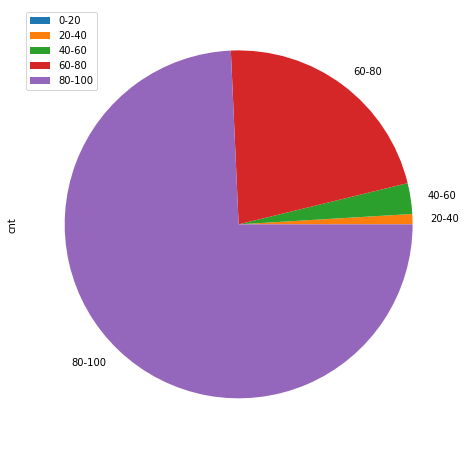
\includegraphics[width=0.4\textwidth]{pie.png}
    \caption{Poměr zastoupení poslanců v kategoriích dle průměrné účasti}
    \label{fig:pie}
\end{figure}

\begin{table}[h!]
    \centering
    \begin{tabular}{lr|lr}
    \hline
        Jméno & účast (\%) & Jméno &        účast (\%) \\
    \hline
        Andrej Babiš &  27.36 & František Navrkal &  100.00 \\
      Karel Schwarzenberg &  32.98 & Jiří Hlavatý &  100.00 \\
        Martin Stropnický &  41.49 & Martin Půta &  100.00 \\
           Milan Chovanec &  45.98 & Radek Rozvoral &   99.73 \\
         Bohuslav Sobotka &  53.21 & Lukáš Bartoň &   99.54 \\
          Antonín Staněk &  56.45 & Miloslav Rozner &   99.54
\end{tabular}
    \caption{Přehled poslanců s nejhorší/nejlepší účastí na hlasováních}
    \label{tbl:mila}
\end{table}

Graf \ref{fig:att_month} zobrazuje průměrnou účast na hlasováních v jednotlivých měsících. Předpokladem bylo, že pokud by účast měla záviset na počasí, potom v letních měsících bude účast menší, než v zimě. To se nepotvrdilo, například v červenci je účast   Střední hodnota účasti na všech hlasováních je $84.69$ \%.

\begin{figure}
    \centering
    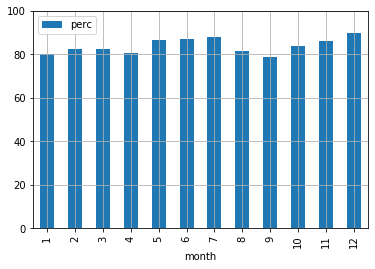
\includegraphics[width=0.7\textwidth ]{images/att_per_month.png}
    \caption{Průměrná přítomnost poslanců v závislosti na měsíci}
    \label{fig:att_month}
\end{figure}

\section{Klasifikace počasí}

Jednou z nejtěžších částí práce bylo určení dní, kdy je hezké počasí. Krom toho, že je označení hezkého dne velice subjektivní záležitost, se mi nepodařilo najít žádnou metodiku, jak takový den programově rozeznat.

Z toho důvodu došlo k vytvoření třech modelů, na kterých byla následně hypotéza ze zadání testována. V prvním modelu je za hezký den považován ten, ve kterém je nadprůměrné počasí. V druhém modelu je za hezký den považován ten, ve kterém je nadprůměrná délka slunečního svitu. Poslední model svým způsobem kombinuje oba předchozí. V něm je jako hezký den určen ten, ve kterém je nadprůměrná teplota, sluneční svit delší, než čtyři hodiny, a nespadli žádné srážky. Procentuální zastoupení v jednotlivých modelech je zobrazen na obrázku \ref{fig:wmodels}.

\begin{figure}
    \begin{subfigure}{.33\textwidth}
        \centering
        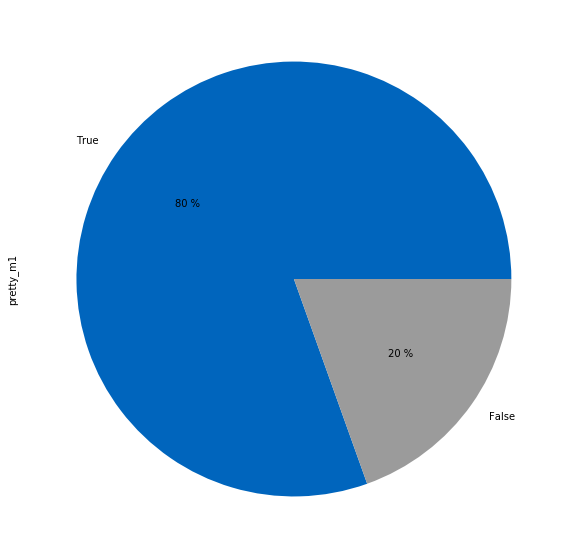
\includegraphics[width=\linewidth]{m1_pie.png}
        \caption{Srážkový model}
        \label{fig:sfig1}
    \end{subfigure}%
    \begin{subfigure}{.33\textwidth}
        \centering
        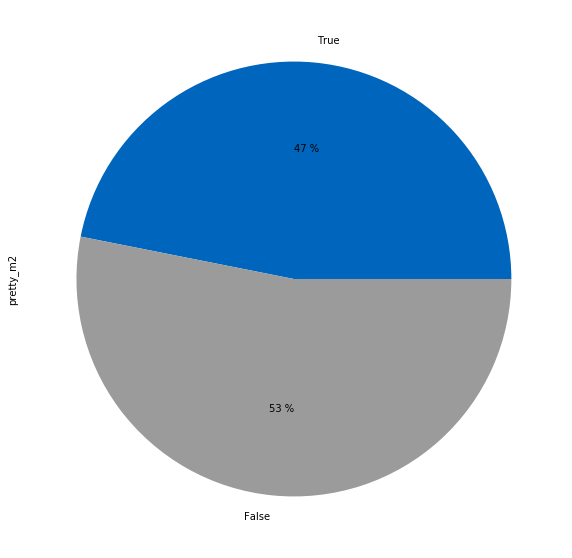
\includegraphics[width=\linewidth]{m2_pie.png}
        \caption{Sluneční model}
        \label{fig:sfig2}
    \end{subfigure}
    \begin{subfigure}{.33\textwidth}
        \centering
        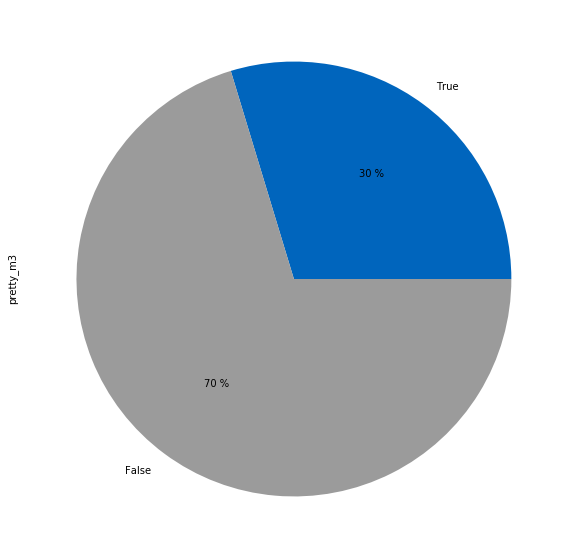
\includegraphics[width=\linewidth]{m3_pie.png}
        \caption{Kombinovaný model}
        \label{fig:sfig2}
    \end{subfigure}
    \caption{Grafy procentuálního zastoupení \uv{hezkých} dnů v jednotlivých modelech}
    \label{fig:wmodels}
\end{figure}

\section{Vztah přítomnosti a počasí}

Na začátek testování hypotézy jsem se pokusil vynést na graf (viz obrázek \ref{fig:weather_att}) normalizovanou neúčast poslanců společně s různými metrikami o počasí. Z grafu ovšem ovšem žádná souvislost mezi veličinami vidět není.

\begin{figure}
    \centering
    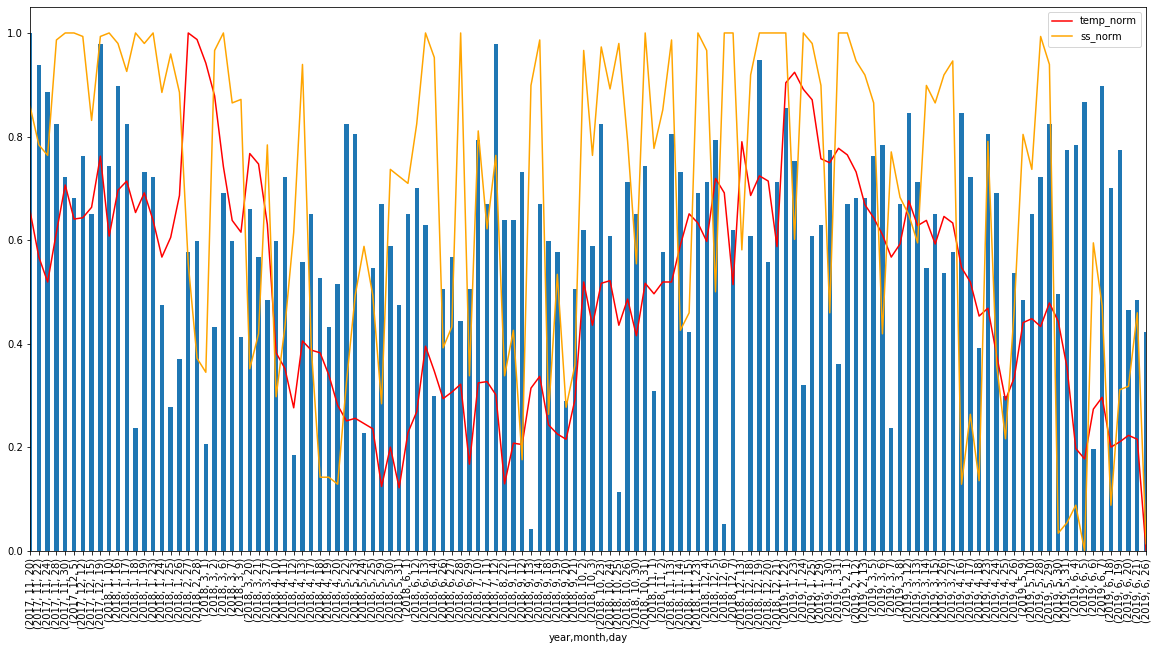
\includegraphics[width=0.75\textwidth]{weather_att.png}
    \caption{Vztah přítomnosti poslanců a různých metrik o počasí}
    \label{fig:weather_att}
\end{figure}

Po vizuální kontrole vztahu veličin jsem přestoupil ke statistickému zpracování data. Pomocí metody \texttt{Point-Biserial Correlation}\footnote{\url{https://en.wikipedia.org/wiki/Point-biserial_correlation_coefficient}} došlo k určení korelace mezi počtem poslanců na hlasováních a počasím. Výsledky pro jednotlivé modely uvádí tabulka \ref{tbl:pm_pd}.

\begin{table}[h!]
    \centering
    \begin{tabular}{lr}
        \hline 
        \textbf{Model} & \textbf{Korelace} \\
        \hline
        Nadprůměrné teploty & -0.020 \\
        Nadprůměrný svit & 0.020 \\
        Kombinovaný model & 0.077
    \end{tabular}
    \caption{Míra korelace mezi počtem lidí v PSP a hezkým dnem}
    \label{tbl:pm_pd}
\end{table}

Z hodnot vypočtených v předchozím kroku vyplývá, že vztah mezi oběma veličinami je zanedbatelný. Proto jsem se rozhodl zkusit zjistit, zda neexistuje vztah mezi přítomností a počasím alespoň u některých jednotlivců.

Pro každého poslance a každý model byla proto metodou \texttt{Rogers–Tanimoto dissimilarity}\footnote{Zhang, Bin and Sargur N. Srihari. \emph{Properties of Binary Vector Dissimilarity Measures.}. 2003.} vypočtena míra odlišnosti mezi nepřítomností a hezkými dny. Výsledky výpočtů uvádí tabulka \ref{tbl:dis}.

\begin{table}[h!]
    \centering
    \begin{tabular}{lr|lr|lr}
                \hline
                Jméno & Odl. & Jméno & Odl. & Jméno & Odl. \\
                \hline
                K. Schwarzenberg &  0.55 & D. Ťok &  0.57 & M. Peksa      &  0.44 \\
                M. Stropnický   &  0.58 & L. Volný     &  0.57 & L. Černohorský  &  0.44 \\
                A. Babiš        &  0.60 & S. Juránek &  0.58 & S. Juránek  &  0.44 \\
                J. Birke           &  0.63 & R. Onderka     &  0.58 & J. Schiller       &  0.45 \\
                A. Staněk      &  0.65 & V. Filip     &  0.59 & M. Oborná      &  0.45 \\
                J. Hamáček         &  0.66 & J. Bláha        &  0.59 & P. Pustějovský  &  0.45 \\
                J. Levová         &  0.68 & M. Bojko      &  0.59 & R. Kubíček      &  0.45 \\
                M. Chovanec      &  0.68 & J. Hamáček       &  0.59 & S. Berkovec &  0.45
            \end{tabular}
    \caption{Míra odlišnosti mezi účastí jednotlivce na hlasováních a \uv{hezkými} dny}
    \label{tbl:dis}
\end{table}

\section{Závěr}

Dle provedených výpočtů a zjištěných skutečností jsem došel k závěru, že přítomnost poslanců v poslanecké sněmovně s počasím nijak výrazně nesouvisí.

\end{document}